% !TeX root = ../main.tex
\section{算力配比的硬件成本表征}
\label{sec:evaluation}

\subsection{实验设置与验证}
\label{sec:eval_setup}
\label{sec:numerical_validation}

九种点积单元以 Verilog 实现，使用 Synopsys Design Compiler X-2025.06 在 TSMC 12\,nm 工艺、TT（0.7\,V、85$^\circ$C）工况下以 1\,GHz 综合，启用集成时钟门控，并通过时序与电气检查。面积统计包含组合逻辑、流水寄存器和门控单元。

功耗评估采用 Qwen3-8B 在 WikiText-2 上运行时第一层 MLP 下投影的激活与权重~\cite{qwen3technicalreport,merity2016pointer}，分别量化为 BF16、MXFP8 E4M3 和 MXFP4 E2M1。Power Compiler 基于 1\,GHz 门级仿真提取的稳态开关活动估计总功耗。面积与功耗均对应综合后、CTS/布局布线前的单 DP。精度验证采用真实模型负载的多精度量化数据，结合随机及边界向量，通过 Verilator 对每种配置完成覆盖 11 种格式的 10,747 笔测试。以独立的精确二进制算术模型为参考，完整计算包含块缩放与累加项 $C$ 的点积，仅在最终结果处按最近偶数舍入至 FP32。在受测数据上，BF16 的最大误差为 3 个 FP32 ULP，其余浮点格式不超过 1\,ULP，其中 HiF4 为 0；INT8/INT32 精确匹配。

\subsection{基线设计与同类多精度单元比较}
\label{sec:related_dp_evaluation}

% Promoted from the approved temporary manuscript.
\suppressfloats[t]
\begin{table}[t]
\centering
\caption{精度支持与组合式配比配置能力。}
\label{tab:related_features}
\begingroup\footnotesize\setlength{\tabcolsep}{1pt}
\def\Y{$\checkmark$}\def\N{$\times$}\def\E{$\triangle$}
\begin{tabular*}{\columnwidth}{@{\extracolsep{\fill}}l*{10}{c}@{}}\toprule
Design & TF32 & FP16 & BF16 & \shortstack{MX\\FP8} & \shortstack{MX\\FP6} & \shortstack{MX\\FP4} & INT8 & \shortstack{NV\\FP4} & HiF4 & \shortstack{Multi\\Ratio} \\\midrule
Ten-Four~\cite{rout2026tenfourv3} & \Y & \Y & \Y & \Y & \N & \N & \Y & \N & \N & \N \\
MXDOTP~\cite{islamoglu2025mxdotp} & \N & \N & \N & \Y & \N & \N & \N & \N & \N & \N \\
FPnew~\cite{mach2021fpnew} & \N & \Y & \Y & \E & \N & \N & \N & \N & \N & \N \\
MiniFloats~\cite{bertaccini2024minifloats} & \N & \Y & \Y & \E & \N & \N & \N & \N & \N & \N \\
TransDot~\cite{transdot2026} & \N & \Y & \N & \E & \N & \E & \N & \N & \N & \N \\
\midrule
DP-Puzzle & \Y & \Y & \Y & \Y & \Y & \Y & \Y & \Y & \Y & \Y \\
\bottomrule\end{tabular*}
\par\smallskip
\parbox{\columnwidth}{\raggedright
$\checkmark$: supported; $\times$: absent in the reported configuration; $\triangle$: element arithmetic supported, integrated MX scaling not established. FPnew and MiniFloats also support FP32/FP64; MiniFloats uses FP8 E5M2/E4M3 and BF16-encoded FP16alt.}
\endgroup
\end{table}

% Generated by scripts/build_related_native.py; official manuscript.
\begin{table*}[t]
\centering
\caption{已有单元与 DP-Puzzle 的原工艺实现条件及效率。}
\label{tab:related_dp}
\begingroup\footnotesize\setlength{\tabcolsep}{1.5pt}
\def\Eff#1{\begin{tabular}{@{}lr@{}}#1\end{tabular}}
\begin{tabular*}{\textwidth}{@{\extracolsep{\fill}}l*{8}{c}@{}}\toprule
Metric & Ten-Four~\cite{rout2026tenfourv3} & MPICC~\cite{huangMPICCMultiplePrecisionInterCombined2025} & MXDOTP~\cite{islamoglu2025mxdotp} & FPnew~\cite{mach2021fpnew} & MiniFloats~\cite{bertaccini2024minifloats} & TransDot~\cite{transdot2026} & \multicolumn{2}{c}{DP-Puzzle} \\
\cmidrule(lr){8-9}
 & & & & & & & $1:2:4$ & $0:2:4$ \\
\midrule
Structure & Fused DP & $n$-term MAC & MX DP & SIMD FMA & SIMD wDotp & FMA / DP & MX DP & MX DP \\
Technology (nm) & 7 & 28 & 12 & 22 & 12 & 12 & 12 & 12 \\
Voltage (V) & 0.7 & 0.9 & 0.8 & 0.8 & 0.8 & 0.8 & 0.7 & 0.7 \\
Frequency (GHz) & 1.58 & 1.43 & 1.09 & 0.923 & 1.26 & 1.0 & 1.0 & 1.0 \\
Area ($\mu$m$^2$) & 2400 / 4650 & 2295 & 3150 & 49\,000 & 19\,000 & $\approx 6000^\dagger$ & 16\,165.12 & 11\,695.21 \\
Accumulation & FP32/INT32 & FP12/INT8 & FP32 & Per format & FP16/FP32 & FP32 & FP32/INT32 & FP32 \\
\midrule
\shortstack[l]{Energy efficiency\\(TFLOP/s/W)} & --- & \Eff{FP8 & 1.948\\FP4 & 5.931} & \Eff{MXFP8 & 2.035} & \Eff{FP16 & 0.498\\BF16 & 0.582\\FP8 & 1.245} & \Eff{FP8 & 1.63\\FP16 & 0.82} & \Eff{FP16 & 0.556\\FP8 & 1.190\\FP4 & 2.439} & \Eff{BF16 & 2.088\\MXFP8 & 4.000\\MXFP4 & 11.432} & \Eff{MXFP8 & 4.713\\MXFP4 & 12.527} \\
\midrule
\shortstack[l]{Area efficiency\\(TFLOP/s/mm$^2$)} & \Eff{BF16 & 5.250 / 5.419\\MXFP8 & 10.500 / 10.839} & \Eff{FP8 & 1.246\\FP4 & 4.985} & \Eff{MXFP8 & 5.524} & \Eff{FP16 & 0.151\\BF16 & 0.151\\FP8 & 0.303} & \Eff{FP8 & 1.06\\FP16 & 0.53} & \Eff{FP16 & $\approx 0.67^{\dagger}$\\FP8 & $\approx 1.33^{\dagger}$\\FP4 & $\approx 2.67^{\dagger}$} & \Eff{BF16 & 1.980\\MXFP8 & 3.959\\MXFP4 & 7.918} & \Eff{MXFP8 & 5.472\\MXFP4 & 10.945} \\
\bottomrule\end{tabular*}
\par\smallskip
\parbox{\textwidth}{\raggedright
均为原工艺数据，不做工艺归一化；支持范围见表~\ref{tab:related_features}。Ten-Four 为全格式 Q8/Q16；MiniFloats 取独立 wDotp FPU，非 cluster。
$\dagger$：TransDot 面积由原文图 7(a) 的 1\,ns 点估读，面效按表 II 吞吐计算；原文相对其 12\,nm FPnew 基线的平均 FP16/FP8 面效为 1.46$\times$/2.92$\times$，不与本表 22\,nm FPnew 值相乘。--- 表示无报告值或不适用。}
\endgroup
\end{table*}


表~\ref{tab:related_features} 与表~\ref{tab:related_dp} 分别比较格式覆盖与实现效率。本文选取 $1:2:4$ 基线作为完整多精度设计的代表，支持 TF32、FP16/BF16、MXFP8/6/4、NVFP4、HiF4 及 INT8，浮点与整型运算分别采用 FP32 和 INT32 累加。相比表中已有单元，该设计在共享通路中覆盖更完整的低精度块缩放格式，兼容 MXFP8/6/4、NVFP4 和 HiF4，并支持多种算力配比，为不同量化方案提供统一的计算基础。

各项效率采用原文报告的工艺与测量条件，以下重点比较同为 12\,nm 的实现。相对 MiniFloats，本文基线的 FP8 面效与能效分别为其 $3.74\times$ 和 $2.45\times$；相对 TransDot，FP8 对应约 $2.97\times$ 和 $3.36\times$，FP4 对应约 $2.97\times$ 和 $4.69\times$。其中，TransDot 的面积由原图估读，相关面效及倍率为近似值，表中以 $\dagger$ 标识。结果表明，完整多精度覆盖与块缩放支持能够兼顾较高的面积和能量效率。

针对采用 7\,nm 工艺的 Ten-Four，表中保留原始数据，正文另用 DeepScaleTool~\cite{sarangi2021deepscaletool} 作工艺缩放比较，以其支持的 14\,nm 节点作为本文 12\,nm 的近似参照。将面积与延迟分别放大 $7.273\times$ 和 $1.132\times$ 后，其全格式 Q8/Q16 配置的 MXFP8 面效估计为 1.275/1.316\,TFLOP/s/mm$^2$，本文 $1:2:4$ 基线为其 $3.10\times$/$3.01\times$。该比较为工艺缩放估算。

针对仅支持低精度计算模式，我们同时列出 $0:2:4$ 低精度专用点积单元设计，以展示格式专用化的收益：在保持 Q32E64 并行度的同时，移除其他精度支持，使 MXFP8 面效由 3.959 提高至 6.555\,TFLOP/s/mm$^2$，能效由 4.000 提高至 5.230\,TFLOP/s/W。按各自原工艺与测量条件比较，相对同为 12\,nm 的 MXDOTP，其 MXFP8 面效提高 18.67\%，能效为其 $2.57\times$，并增加 MXFP4、NVFP4 和 HiF4 支持。相对 28\,nm 的 MPICC，FP8 面效与能效分别为其 $5.26\times$ 和 $2.68\times$，FP4 分别为 $2.63\times$ 和 $2.35\times$。采用上述工艺缩放方法，相对 Ten-Four 的 MXFP8 专用 Q8/Q16 配置，本文 $0:2:4$ 的 MXFP8 面效分别为其 $2.15\times$/$2.10\times$，同时保留 FP4 计算支持。

\subsection{九种配比的面积与功耗}
\label{sec:lowp_costs}

图~\ref{fig:ratio4_costs} 给出九种配比的面积与总功耗，面积倍率以 $1:2:4$ 为参照，功耗直接报告 mW。以下各模式增幅均与基线的同精度功耗比较。$1:2:6$ 和 $1:2:8$ 分别将 E 算力提高 50\% 和 100\%，DP 面积仅增加 16.69\% 和 33.60\%，E 模式功耗增加 28.77\% 和 57.14\%。两者的 H/Q 模式功耗增幅均低于 4\%，表明共享后端与按模式激活能够限制增配资源对其他精度的影响。

$1:4:8$ 将 Q/E 算力同时翻倍，面积增加 68.21\%；Q 和 E 模式功耗分别增加 79.91\% 和 83.66\%，H 模式仅增加 2.71\%。其 Q 模式总功耗为 28.789\,mW。与 E 专用增配相比，QE Group 还需保留 Q 的指数比较、局部对齐及宽规约通路，因而具有更高成本。

更大增配进一步展开了成本差异。$1:2:12$ 和 $1:2:16$ 将 E 容量提高至基线的 3 倍和 4 倍，面积分别增加 64.68\% 和 83.68\%，E 功耗增加 109.56\% 和 162.42\%。只增强 Q 的 $1:4:4$ 面积增加 48.56\%，低于共同增配的 $1:4:8$。$1:6:12$、$1:8:16$ 的面积增幅分别为 136.52\% 和 190.29\%，Q 模式功耗达到 41.351 和 52.853\,mW；九种配置的 H 功耗增幅均不超过 6.27\%。

\begin{figure*}[t]
\centering
{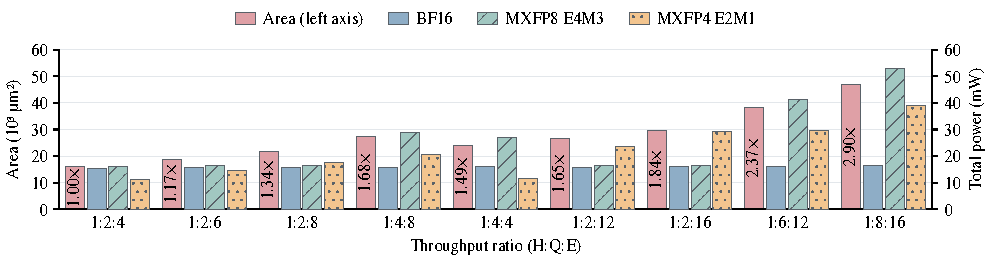
\includegraphics[width=2\columnwidth]{dp_ratio_area_power.pdf}}
\caption{九种配比的综合面积与总功耗。面积柱按左轴读取，标签为相对 $1:2:4$ 的倍率；三种精度的功耗柱按右轴读取（mW）。}
\label{fig:ratio4_costs}
\end{figure*}

\textbf{观察一：算力、面积与功耗不按同一比例增长。} E 专用通路能以较小成本提高 E 吞吐，而同时提高 Q 吞吐需要更多对齐与规约资源。因此，配比 DSE 应使用各候选的面积和逐模式功耗，不能按峰值比例线性放大基线成本。

\subsection{持续供数所需的带宽}
\label{sec:ratio_bandwidth}

考虑固定的 $m\times n$ DP 阵列：A 沿行广播并在本地寄存器中复用 $x$ 个周期，B 沿列广播且每周期更新。每个 DP 每拍处理 $K$ 项乘积，频率为 $f$，同一精度下每元素占 $b$ 位（含均摊尺度开销），则 shared memory 向阵列提供输入的稳态平均带宽需求为
\begin{equation}
B_{\mathrm{in}}(K,x)=fbK\left(\frac{m}{x}+n\right),\qquad
\frac{B_{\mathrm{in}}(K_j,x)}{B_{\mathrm{in}}(K_0,x)}=\frac{K_j}{K_0}.
\label{eq:ratio_bandwidth}
\end{equation}
这里固定阵列尺寸、频率及复用周期，并假设完整缩放块下输入位数随 $K$ 同比增长。A 的复用降低了重复读取开销，但每周期更新的 B 仍需持续供给。因此，相比 $1:2:4$，$1:2:8$ 的 E 模式、$1:4:8$ 的 Q/E 模式在满吞吐下均需要约两倍输入带宽。增配低精度算力时，需要同时考虑 shared memory 的供给是否跟得上阵列消费；后续 DSE 仍以供数充分为前提，不加入 shared memory 带宽约束。
